\usecasegenerico{Visualizzazione elenco ristoranti}
\label{usecase:Visualizzazione elenco ristoranti}

\begin{figure}[h]
	\centering
	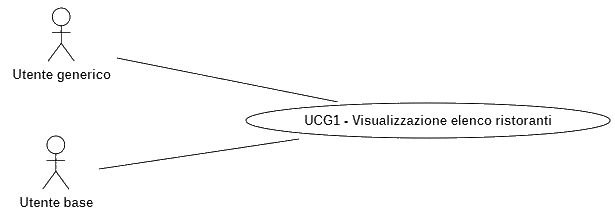
\includegraphics[width=0.8\textwidth]{./uml/UCG1.png} 
	\caption{Visualizzazione elenco ristoranti}
	\label{fig:UCG1}
  \end{figure}

\begin{itemize}
	\item \textbf{Attore principale:} Utente generico.

	\item \textbf{Precondizione:}
	      L'utente è connesso al Sistema.

	\item \textbf{Postcondizione:} L'Utente generico visualizza una lista di
	      ristoranti. Di \textit{default} la lista viene presentata in ordine decrescente di valutazione.

	\item \textbf{Scenario principale:}
	      \begin{enumerate}
		      \item L'Utente generico seleziona la funzionalità di
		            visualizzazione dei ristoranti;

		      \item il Sistema presenta all'utente un elenco di ristoranti disposti in ordine decrescente di valutazione media;

		      \item L'Utente generico visualizza la lista dei ristoranti secondo tale visualizzazione.

	      \end{enumerate}
\end{itemize}
